\lstnewenvironment{Cpp}[1][]		% fuer C++-Code
  {\lstset{
  	backgroundcolor=\color{black!5},    % choose the background color
    language=C++,			
    basicstyle=\footnotesize\ttfamily,	% basic font setting
    breaklines=true,
    frame=none,
    numbers=left,						% where to put the line-numbers
    numbersep=5pt,						% how far the line-numbers are from the code
    stepnumber=1,						% the step between two line-numbers.
    tabsize=4,                      	% sets default tabsize to 2 spaces
	showspaces=false,               	% show spaces adding particular underscores
	showstringspaces=false,         	% underline spaces within strings
	showtabs=false,                	 	% show tabs within strings adding particular underscores
    breaklines=true,                	% sets automatic line breaking
    breakatwhitespace=true,        	 	% sets if automatic breaks should only happen at whitespace
    keywordstyle=\color[rgb]{0.627451,0.125490,0.941176},		% Purple
    commentstyle=\color[rgb]{0.133333,0.545098,0.133333},		% forest green
    stringstyle=\color[rgb]{0.803922,0.360784,0.360784},		% indian red 
    numberstyle=\color[rgb]{0.019608,0.019608,0.019608},		% grey 
    literate={0}{{\textcolor{blue}{0}}}{1}%
             {1}{{\textcolor{blue}{1}}}{1}%
             {2}{{\textcolor{blue}{2}}}{1}%
             {3}{{\textcolor{blue}{3}}}{1}%
             {4}{{\textcolor{blue}{4}}}{1}%
             {5}{{\textcolor{blue}{5}}}{1}%
             {6}{{\textcolor{blue}{6}}}{1}%
             {7}{{\textcolor{blue}{7}}}{1}%
             {8}{{\textcolor{blue}{8}}}{1}%
             {9}{{\textcolor{blue}{9}}}{1}%
        	 ,
  }}{}

\chapter{Kugelsternhaufen}
\lhead{Kugelsternahufen}
\begin{refsection}
\chapterauthor{Flavio La Morea und Nicol\'as Rom\'an L"uthold}

\section{Grundlagen}
\rhead{Grundlagen}

\subsection{Einf"uhrung}
\begin{minipage}{.65\textwidth}
\index{Kugelsternhaufen}
Kugelsternhaufen sind eine Ansammlung sehr vieler Sterne, die kugelf"ormig
untereinander gravitativ gebunden sind. Mehrere 100'000 Sterne kann
man hierbei als typisch bezeichnen. Die Sterne sind vorwiegend alte,
rote Sterne d.h. sie enthalten nur wenige schwere Elemente. Die
durchschnittliche Sternendichte betr"agt 0,4 Sterne pro Kubikparsec (1
Parsec entspricht ca. 3,26 Lichtjahren $\mathrm{= 3,086 \cdot 10^{16}
m}$). Im Kern ist die Dichte allerdings viel h"oher mit 100 bis 1000
Sternen pro Kubikparsec.
\index{Lichtjahr}
\index{Stern}
\index{Parsec}
\index{Kubikparsec}

Unser Auftrag bestand darin die Bewegung der Sterne in einem
Kugelsternhaufen zu simulieren. \cite{kugel:wiki:grundlagen}
\end{minipage}
\hspace{.5cm}
\begin{minipage}{.3\textwidth}
\begin{center}
	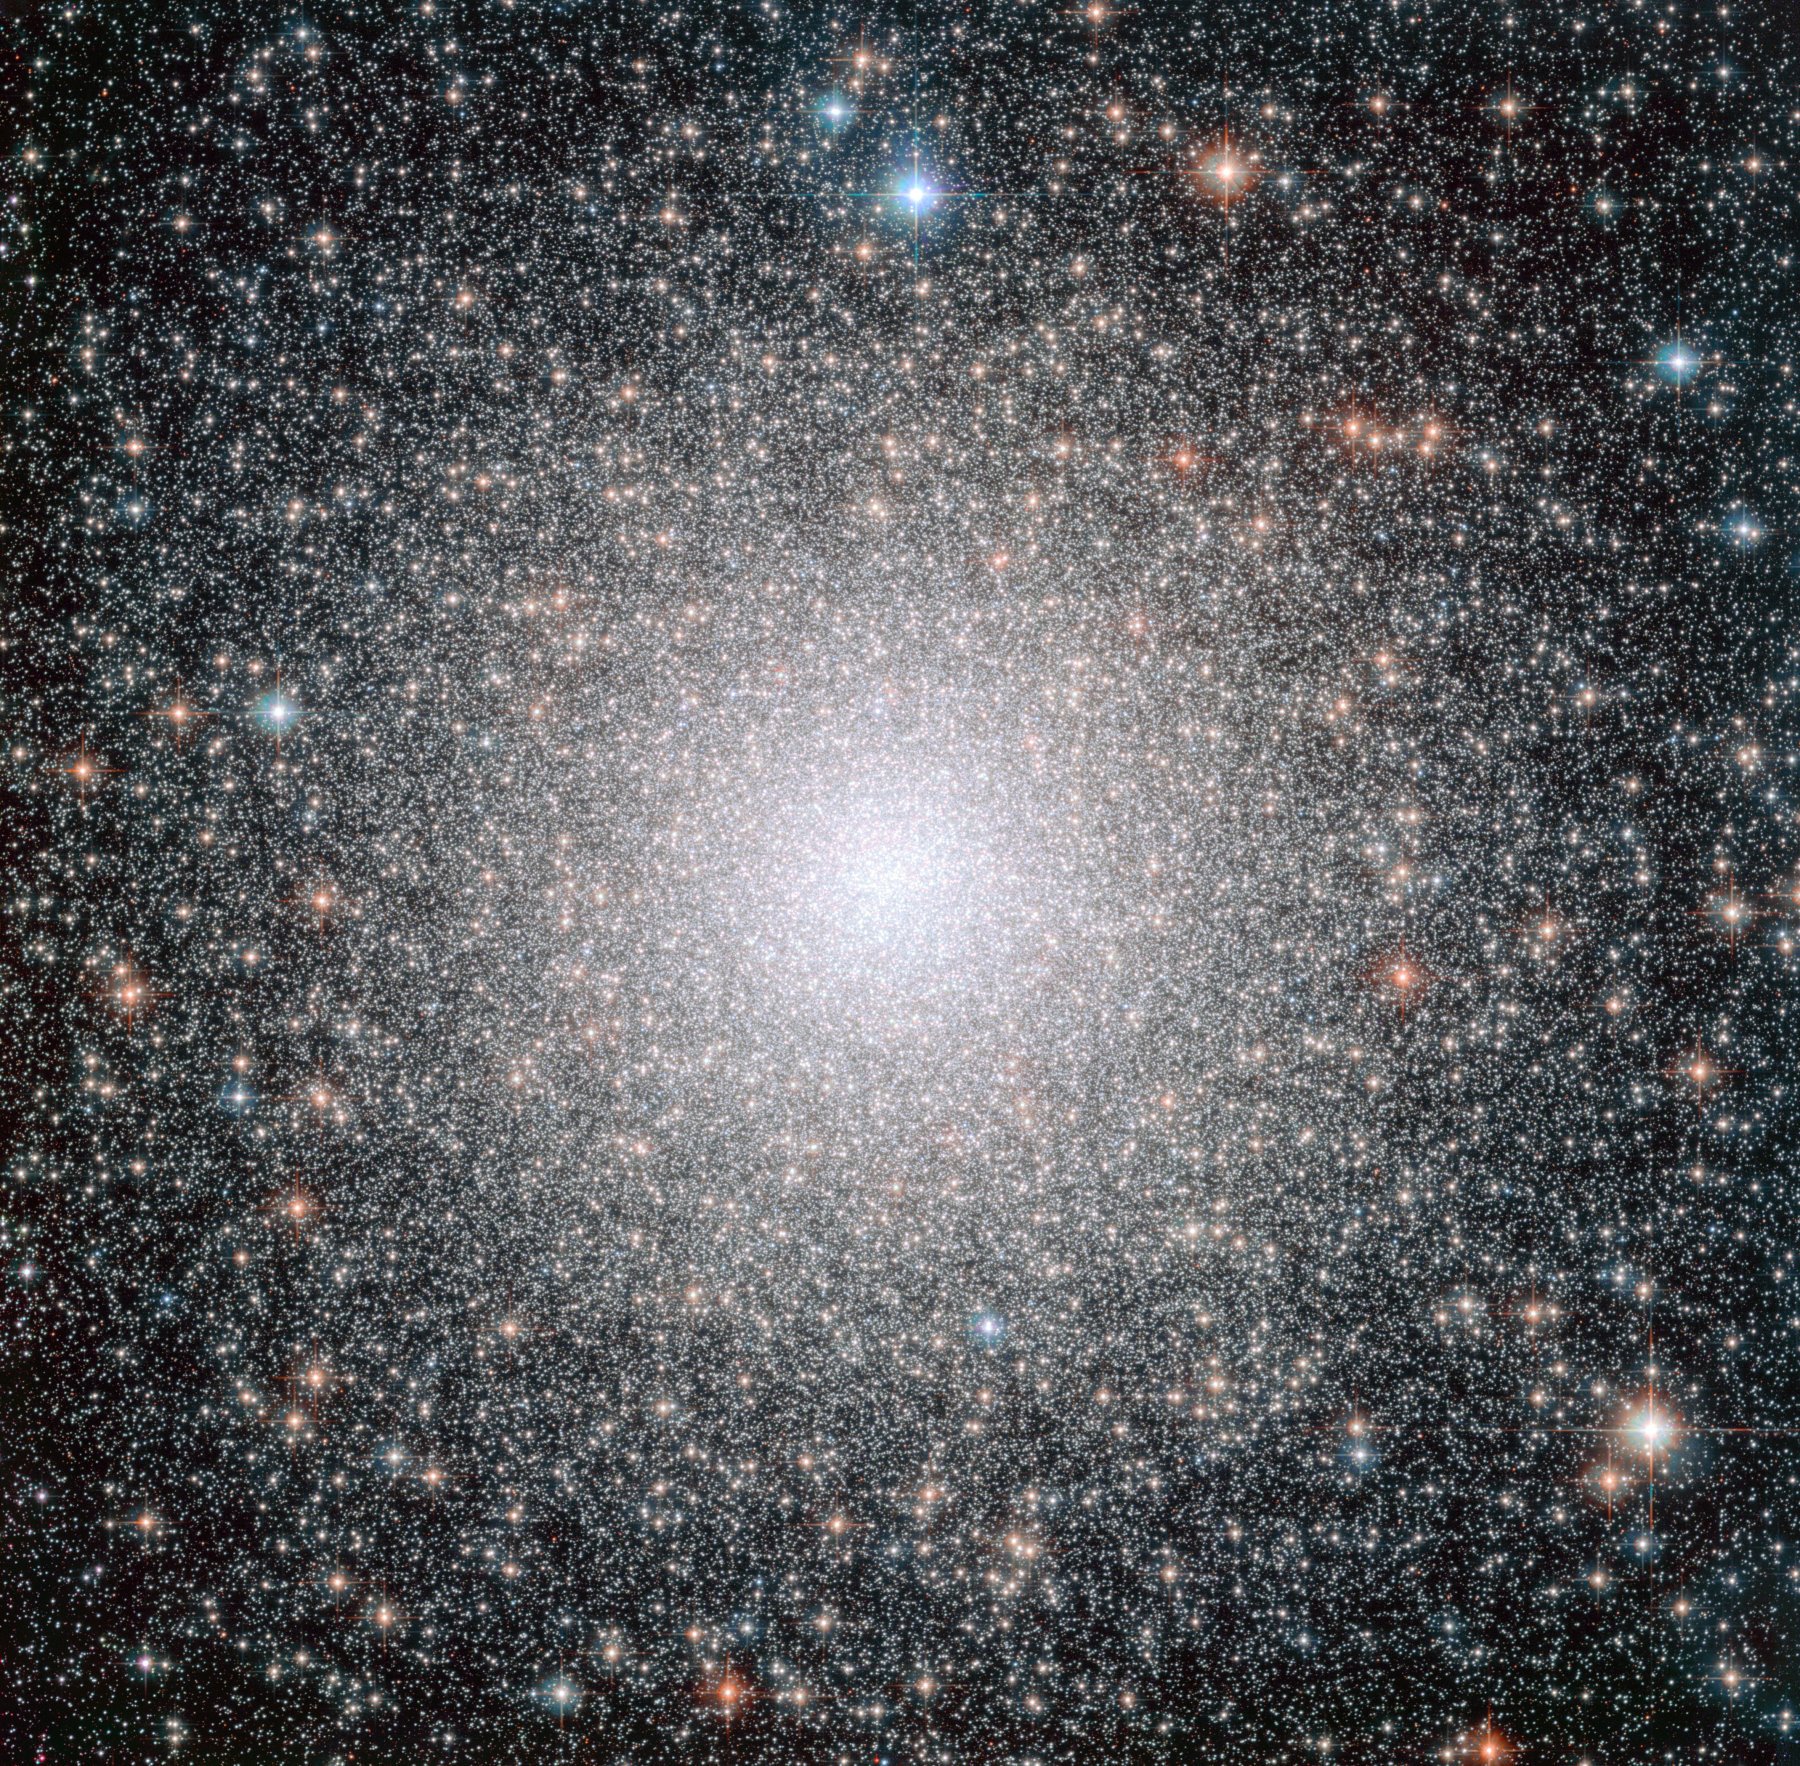
\includegraphics[width = \textwidth]{kugel/images/Abbildung1_1.jpg}
	Kugelsternhaufen NGC 6388 \cite{kugel:titelbild}
\end{center}
\end{minipage}
\index{NGC 6388}

\subsection{Berechnung der gravitativen Krafteinwirkung auf einen Stern} \label{kugel:subsection:Kraftformel}
F"ur unsere Simulation gen"ugt es die Sterne als Massenpunkte zu behandeln. 
Die gravitative Kraftwirkung zwischen zwei Massenpunkten l"asst sich
mit Hilfe des newtonschen Gravitationsgesetzes berechnen:
\index{Gravitationsgesetz}
\begin{equation}
	F = G \cdot \dfrac{m_i m_j}{r^2}
	\label{kugel:Formel:NewtonGrav}
\end{equation}
$F$: Betrag der Kraft zwischen zwei Massenpunkten (Sternen) \\
$m_i$: Masse des Sterns $i$ \\
$m_j$: Masse des Sterns $j$ \\
$r$: Abstand zwischen den beiden Sternen \\
$\mathrm{G = 6,67384 \cdot 10^{-11} \frac{m^3}{kg \cdot s^2}}$
ist die Gravitationskonstante \\ \\
In unserer Simulation wird in drei Dimensionen gerechnet, daher schreiben
wir nun die Formel (\ref{kugel:Formel:NewtonGrav}) in eine vektorielle
Form um:
\begin{equation}
	F_{ji} = G \dfrac{m_i m_j}{\lvert x_i -  x_j \lvert^2} \dfrac{x_i - x_j}{\lvert x_i - x_j \lvert}
	\label{kugel:Formel:NewtonGravVek}.
\end{equation}
$F_{ji}$: Kraftvektor der auf den Stern $j$ beschleunigend wirkt \\
$m_i$: Masse des Sterns $i$ \\
$m_j$: Masse des Sterns $j$ \\
$x_i$: Positionsvektor des Sterns $i$ \\
$x_j$: Positionsvektor des Sterns $j$  \\ \\
$\displaystyle \frac{ x_i -  x_j}{\lvert  x_i -  x_j \lvert}$ dient
dabei als Richtungsvektor.
	
So wird nur die Kraftwirkung eines einzelnen Sterns $i$ auf den Stern
$j$ berechnet.
Daher summieren wir alle Kr"afte $F_{ji}$, die auf den Stern $j$ wirken:
\begin{equation}
	 F_j = \sum_{j \neq i} F_{ji} = G \sum_{j \neq i} \dfrac{m_i m_j}{\lvert x_i - x_j \lvert^2} \dfrac{x_i - x_j}{\lvert x_i - x_j \lvert}
	\label{kugel:Formel:NewtonGravVekSum}.
\end{equation}
$F_j$ beschreibt die Kraft mit der alle anderen Sterne des Haufens
gravitativ auf den Stern $j$ wirken.
Durch $F_j$ wird die Sternbewegung vollst"andig bestimmt.
		
\subsection{Differentialgleichung der Sternbewegung}
Das zweite Newtonsche Gesetz sagt uns, dass:	
\begin{equation}
	 F = m  a = m \ddot{x}.
	\label{kugel:Formel:Newton2}
\end{equation}
Jetzt setzen wir in dieser Gleichung f"ur $F$ die Kraftformel
(\ref{kugel:Formel:NewtonGravVekSum}) ein. Dadurch erhalten wir eine
Differentialgleichung zweiter Ordnung. "Ublicherweise schreibt man
Differentialgleichungen in folgender Form auf:
\[
\text{H"ochste Ableitung der Funktion} = \text{Term mit der Funktion drin}
\]
Bringt man die Differentialgleichung (\ref{kugel:Formel:Newton2}) in
diese Form, erh"alt man:
\begin{equation}
\ddot{{x_j}} = \dfrac{G}{m_j} \sum_{j \neq i} \dfrac{m_i m_j}{\lvert  x_i -  x_j \lvert^2} \dfrac{x_i -  x_j}{\lvert x_i -  x_j \lvert}.
\label{kugel:Formel:DGLo2}
\end{equation}
$x_j$ ist die Position des Sterns $j$, sie ist als Funktion der Zeit
zu verstehen.
	
Numerische L"osungsverfahren werden im Normalfall f"ur Systeme erster
Ordnung formuliert.
Somit muss die Ordnung unserer Differentialgleichung noch reduziert
werden.
Dies geschieht durch eine Umwandlung in ein Differentialgleichungssystem
erster Ordnung.
Zur Umwandlung nehmen wir die Geschwindigkeit des Sterns $j$ hinzu,
also die Funktion $v_j = v_j(t) = \dot{x_j}$.
Zusammen mit $\ddot{x_j} = \dot{v_j}$ erhalten wir jetzt die folgenden
Differentialgleichungen erster Ordnung:
\begin{equation}
\begin{aligned}
	\dot{v_j} &= \dfrac{G}{m_j} \sum_{j \neq i} \dfrac{m_i m_j}{\lvert x_i - x_j \lvert^2} \dfrac{x_i - x_j}{\lvert x_i - x_j \lvert} \\
	\dot{x_j} &= v_j
\end{aligned}
\label{kugel:Formel:DGLSys}
\end{equation}
Dieses neue Differentialgleichungssystem soll als n"achstes numerisch
gel"ost werden.
	
\subsection{Numerische L"osung}
Zur L"osung des Anfangswertproblems haben wir das explizite
Euler-Verfahren gew"ahlt. Hierbei handelt es sich um das einfachste
\index{Euler-Verfahren}
Verfahren f"ur numerische L"osungen von Anfangswertproblemen. Dieses
wird nun kurz erl"autert, als Beispiel nehmen wir die einfache
Differentialgleichung:
\begin{equation}
\dot{y} = f(t,y)
\label{kugel:Formel:DGLbsp}
\end{equation}
Wenn der Wert der L"osung f"ur einen bestimmten anfänglichen Zeitpunkt
$t_0$ bekannt ist, dann kann man die L"osung f"ur den n"achsten Zeitpunkt
$t_0 + dt$ n"aherungsweise durch lineare Approximation berechnen:
\begin{equation}
y(t_0 + dt) = y(t_0) + dt \cdot f(y(t_0))
\label{kugel:Formel:EulerAllg}
\end{equation}
Damit unser System also gel"ost werden kann, sind initiale Werte f"ur
Positionen und Geschwindigkeiten der Sterne notwendig.
Wie diese Anfangswerte in unserer Simulation initialisiert werden,
wird in den Abschnitten \ref{kugel:subsection:InitMasse} und
\ref{kugel:subsection:InitPosGesch} gezeigt. Das Euler-Verfahren liefert
dann folgende Approximation der zwei L"osungsfunktionen:
\begin{equation}   
\begin{aligned}
x_{j,n+1} &=  x_{j,n} + dt \cdot  v_n \\
     v_{j,n+1} &=  v_{j,n} + dt \cdot \dfrac{G}{m_j} \sum_{j \neq i} \dfrac{m_i m_j}{\lvert x_i - x_j \lvert^2} \dfrac{x_i - x_j}{\lvert x_i - x_j \lvert}
\end{aligned}
\label{kugel:Formel:EulerSys}
\end{equation}
Die berechneten Werte stellen dabei Approximationen an die tats"achlichen
Werte der exakten L"osung des Anfangswertproblems dar. Je kleiner die
Schrittweite $dt$ gew"ahlt ist, desto mehr Rechenarbeit ist n"otig,
aber desto genauer werden auch die approximierten Werte.
Wir haben das Verfahren wegen dem geringen Rechenaufwand gew"ahlt, es
g"abe noch wesentlich genauere (z.B. das Runge-Kutta) deren Rechenaufwand
\index{Runge-Kutta-Verfahren}
deutlich h"oher, aber das Problem der Schrittweite immernoch vorhanden
w"ar.

\subsection{Wahl des Zeitschritts}
Die Wahl der Schrittweite $dt$ f"ur einen Euler-Schritt hat sich
\index{Euler-Schritt}
\index{Schrittweite}
als besonders schwierig herausgestellt. Sie bestimmt die Intervalle
in denen die aktuelle Position eines Sterns aktualisiert wird,
d.h. dass die Flugbahn eines Sterns schrittweise berechnet wird. Ein
k"urzerer Zeitschritt liefert eine bessere Genauigkeit, verlangt aber
mehr Rechenschritte f"ur die gleiche simulierte Zeitspanne oder mehr
Rechenzeit. Um eine m"oglichst lange Zeitspanne simulieren zu k"onnen,
versucht man den Zeitschritt m"oglichst gross zu machen.
    
Andererseits sp"uren die Sterne nur dann eine merkliche Kraft, wenn sie
sich gen"ugend nahe sind. Sich schnell bewegende Sterne sind aber nur eine
sehr kurze Zeit nahe beieinander, man muss also den Zeitschritt k"urzer
als die Begegnungszeit von zwei Sternen w"ahlen. Tut man dies nicht,
fliegen die simulierten Sterne einfach aneinander vorbei, wie wenn es
"uberhaupt keine Schwerkraft g"abe.
     
\section{Implementation}
\rhead{Implementation}
F"ur die Simulation wurde ein C++ Programm erstellt. Es kann
bei Interesse unter diesem GitHub Repository bezogen werden:
\url{https://github.com/nromanlu/Kugelsternhaufen}.
Folgend ein paar Informationen zu unserer Implementation.

\subsection{Klasse Stern}
Die Klasse \texttt{Stern} ist der Hauptbestandteil des Programms. Objekte, also Sterne, enthalten jeweils folgende drei Eigenschaften:
\begin{Cpp}
double m;			// Masse in kg
double v[3];		// Geschwindigkeit in m/s
double pos[3];		// Positon in m 
\end{Cpp}
Ebenfalls beinhaltet die Klasse eine Methode namens \texttt{run1s},
welche die neue Position, Richtungs- sowie Geschwindigkeitseinfluss eines
Sterns w"ahrend einem Zeitschritt berechnet. Dies geschieht durch L"osen
des bereits erw"ahnten Gleichungssystem \ref{kugel:Formel:EulerSys},
was im Code so aussieht:
\begin{Cpp}
for(int i = 0 ; i < AnzSt ; i++){	// Einfluss aller Sterne
	if (i != stern) {				// ausser der aktuelle Stern
		Anz = G*m*haufen[i].m;
		Dist = getDistance(&haufen[i].pos[0]);
		DistPow = pow(Dist, 2);

		// Wirkenden Kraftvektor ausrechen
		f[0] -= (Anz*(pos[0]-haufen[i].pos[0]))/(DistPow*Dist);
		f[1] -= (Anz*(pos[1]-haufen[i].pos[1]))/(DistPow*Dist);
		f[2] -= (Anz*(pos[2]-haufen[i].pos[2]))/(DistPow*Dist);
	}
}
// Neue Position
pos[0] += dt*v[0];
pos[1] += dt*v[1];
pos[2] += dt*v[2];

// Richtungs- und Geschwindigkeitseinfluss auf den Stern
v[0] += dt*f[0]/m;
v[1] += dt*f[1]/m;
v[2] += dt*f[2]/m;
\end{Cpp}
	
\subsection{Initialisierung der Masse \label{kugel:subsection:InitMasse}}
Die typische Masse eines Sternes in einem Kugelsternhaufen entspricht
etwa der unserer Sonne ($\mathrm{1.989 \cdot 10^{30} kg}$). Allerdings
haben wir uns f"ur eine um ca. Faktor 100 kleinere Masse entschieden,
welche im Programm wie folgt initialisiert wird:
\begin{Cpp}
m = ((rand()%100)+50)*1e25; 
\end{Cpp}
\texttt{rand()  \% 100} liefert zuf"allige gleichverteilte Zahlen
zwischen 0 und 99, der Rest sollte selbsterkl"arend sein. Sternmassen
sind normalerweise nicht gleichverteilt, sondern eher so wie im
Herzsprung-Russel-Diagramm beschrieben. Dabei stellten wir fest, dass eine
zu grosse Streuung der Sternmassen sich negativ auf den Kugelsternhaufen
auswirken kann.\\
\begin{figure}[h!]
	\begin{center}
		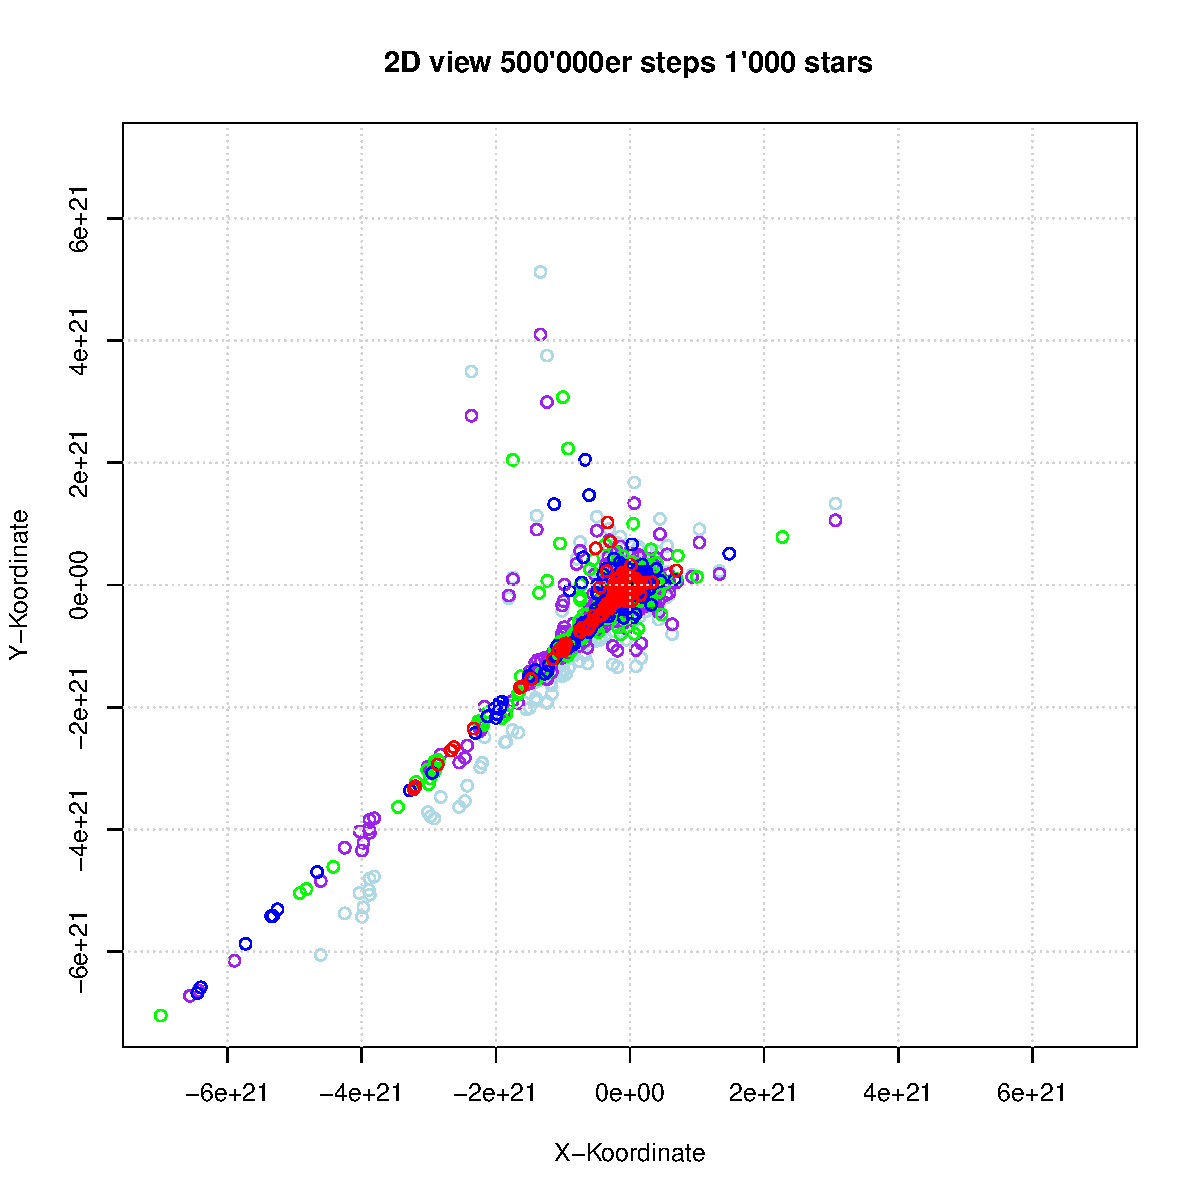
\includegraphics[width = 8cm]{kugel/images/lolli.pdf}
	\end{center}
	\caption{Massenproblem
	\label{Kugel.Massenproblem}}
\end{figure}

Bei diesem Beispiel der Abbildung~\ref{Kugel.Massenproblem} ist ein
grosser Stern aus dem Haufen rausgeflogen und hat dabei andere Sterne
hinterher gezogen. Eine Gleichverteilung war uns schlussendlich als
Basis f"ur die Simulation eine akzeptable erste N"aherung.
	
\subsection{Initialisierung von Position und Geschwindigkeit \label{kugel:subsection:InitPosGesch}}
Die Entstehung eines Kugelsternhaufens ist noch nicht wirklich weit
erforscht, was die Wahl der Anfangsbedingungen erschwerte. Wie die Masse
eines Sternes initialisiert wird wissen wir bereits, doch wie sieht es
mit der Position und Geschwindigkeit aus? Die anf"angliche Position der
Sterne wird durch folgende Formel berechnet:
\begin{Cpp}
int ZahlenBereich = 10000;
pos[0] = ((ZahlenBereich/2) - ((rand()%ZahlenBereich)+1))*1e15; 
pos[1] = ((ZahlenBereich/2) - ((rand()%ZahlenBereich)+1))*1e15; 
pos[2] = ((ZahlenBereich/2) - ((rand()%ZahlenBereich)+1))*1e15; 
\end{Cpp}
Als Zufallszahlgenerator wurde wieder die rand()-Funktion verwendet. Die
\index{Zufallszahlen}
m"oglichen Werte f"ur die Positionen befinden sich zwischen $\mathrm{\pm5
\cdot 10^{18} m}$. Wir haben diesen Wert gew"ahlt damit die Sterne anfangs
relativ nahe aufeinander liegen und sofort die gravitative Wirkung
ersichtlich ist. Ein 2D-Plot (Abbildung~\ref{Kugel:Anfangspossition})
der Anfangspositionen zeigte auf, dass die Sterne sich gleichverteilt
in einem Quadrat aufteilen was man als Problem ansehen kann.

\begin{figure}[h!]
	\begin{center}
		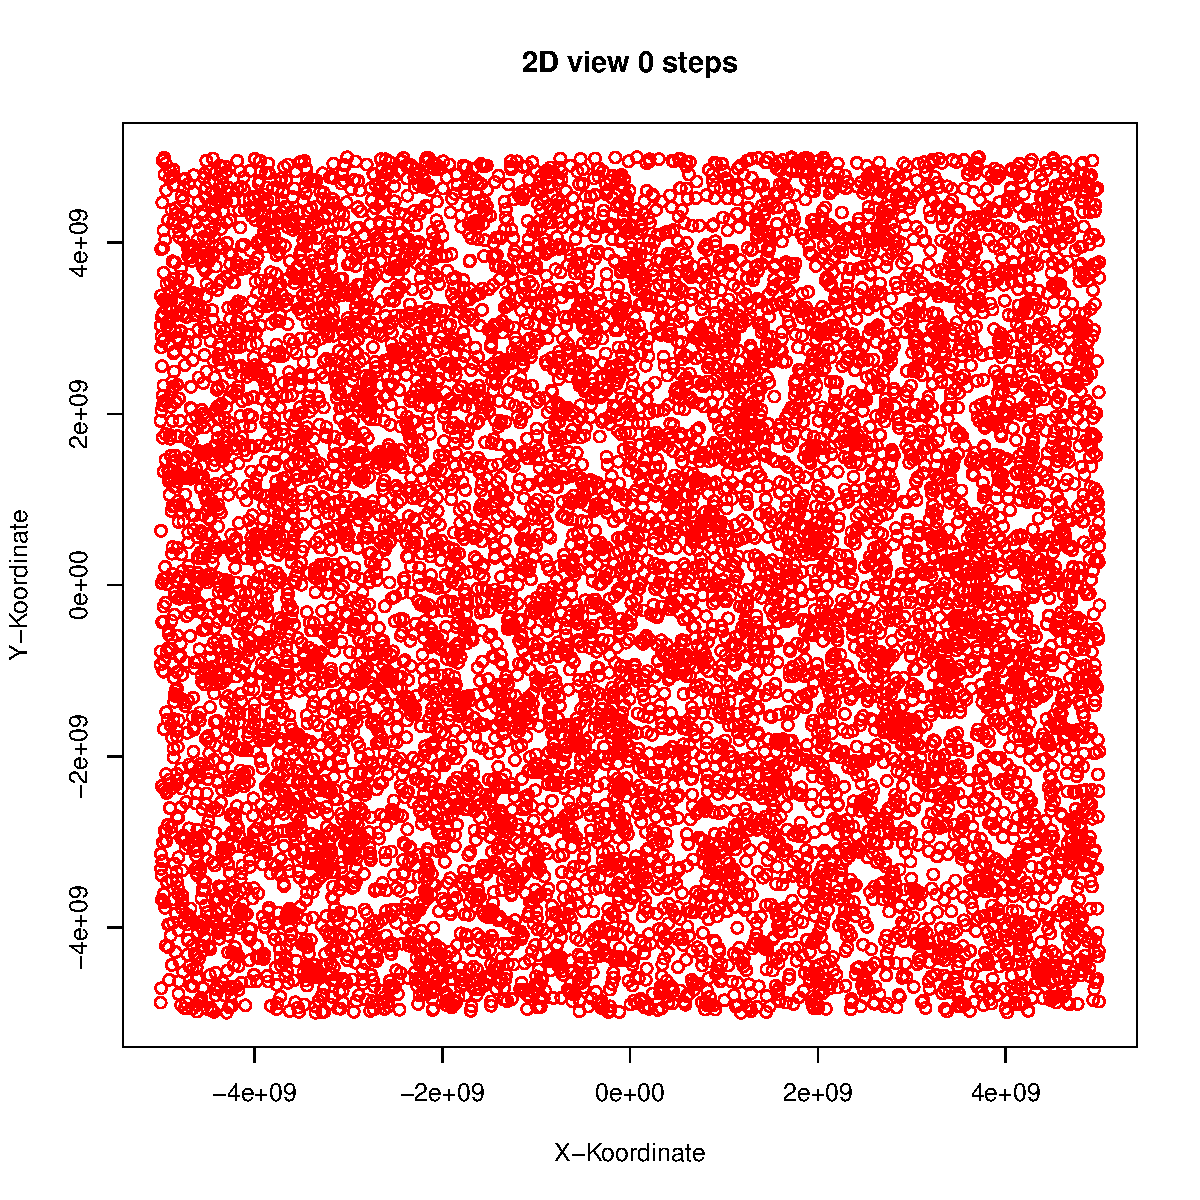
\includegraphics[width = 8cm]{kugel/images/2DPosN0.pdf}
	\end{center}
	\caption{Anfangspositionen 2D
	\label{Kugel:Anfangspossition}}
\end{figure}

Die Anfangsgeschwindigkeiten wurden ebenfalls per rand()-Funktion (also
wieder gleichverteilt) berechnet:
\begin{Cpp}	
double gesch = 20;
v[0] = ((rand()%ZahlenBereich)+1)/gesch;
v[1] = ((rand()%ZahlenBereich)+1)/gesch; 
v[2] = ((rand()%ZahlenBereich)+1)/gesch;
\end{Cpp}
Der Intervall der m"oglichen Werte ist hierbei $\mathrm{1 - 5000
\frac{m}{s}}$. Dieser wurde experimentell durch Auswerten mehrerer
Simulationen bestimmt. Durch diese einfachen Initialisierungen kommt
der Kugelsternhaufen in eine initiale Phase, in der er dann erst seine
``Form"' finden muss.
	
\subsection{Parallelisierung}
In unserem Code gibt es zwei ineinander verschachtelte for-Schleifen. Die
"Aussere ist nur f"ur die Zeitschritte und die Innere f"ur die Sterne
selber.
\begin{Cpp}
for(int j=0 ; j<steps ; j++){              // Anz. Zeitschritte
  #pragma omp parallel for num_threads(32) // Parallelisierung
  for(int i=1 ; i< anzahlSterne ; i++) {   // F"ur jeden Stern
    s[i].run1s(s, anzahlSterne, i);		   // 1 Zeitschritt
  }										   // abarbeiten	
}
\end{Cpp}
Es ist dabei sinnlos bzw. sogar unm"oglich f"ur unsere Simulation die
"aussere Schleife zu parallelisieren.
    
In der inneren for-Schleife werden parallel, Zeitschritt f"ur Zeitschritt
alle Sterne abgearbeitet. Zur Parallelisierung dieser Schleife ist
OpenMP die einzig richtige Wahl. Es gibt keine sinnvolle Unterteilung
des Problemgebietes f"ur eine Parallelisierung mit OpenMPI (jedes Teil
m"usste den Mittelpunkt enthalten), und OpenCL kommt nicht in Frage, weil
alle Threads nach jedem Zeitschritt wieder synchronisiert werden m"ussten.

Die Implementierung von OpenMP in unseren Code war sehr einfach, es
\index{OpenMP}
wurde lediglich nur eine Zeile mehr Code gebraucht.
\begin{Cpp}
#pragma omp parallel for num_threads(32)
\end{Cpp}
\index{numthreads@\texttt{num\_threads}}
Mehr als 32 Threads zu w"ahlen war zwecklos, weil bei unserem Cluster
nur 32 FPUs vorhanden sind.
    
\subsection{Impulskorrektur}
Nach den ersten paar Versuchen bemerkten wir dass der Kugelsternhaufen
am ``wegfliegen"' war. Dies sieht man sch"on auf dem Plot der
Abbildung~\ref{Kugel.Impulsproblem}. Der Verlauf der Position des Haufens
ist mit verschiedenen Farben dargestellt (beginnend bei Rot).
\begin{figure}[h]
	\begin{center}
		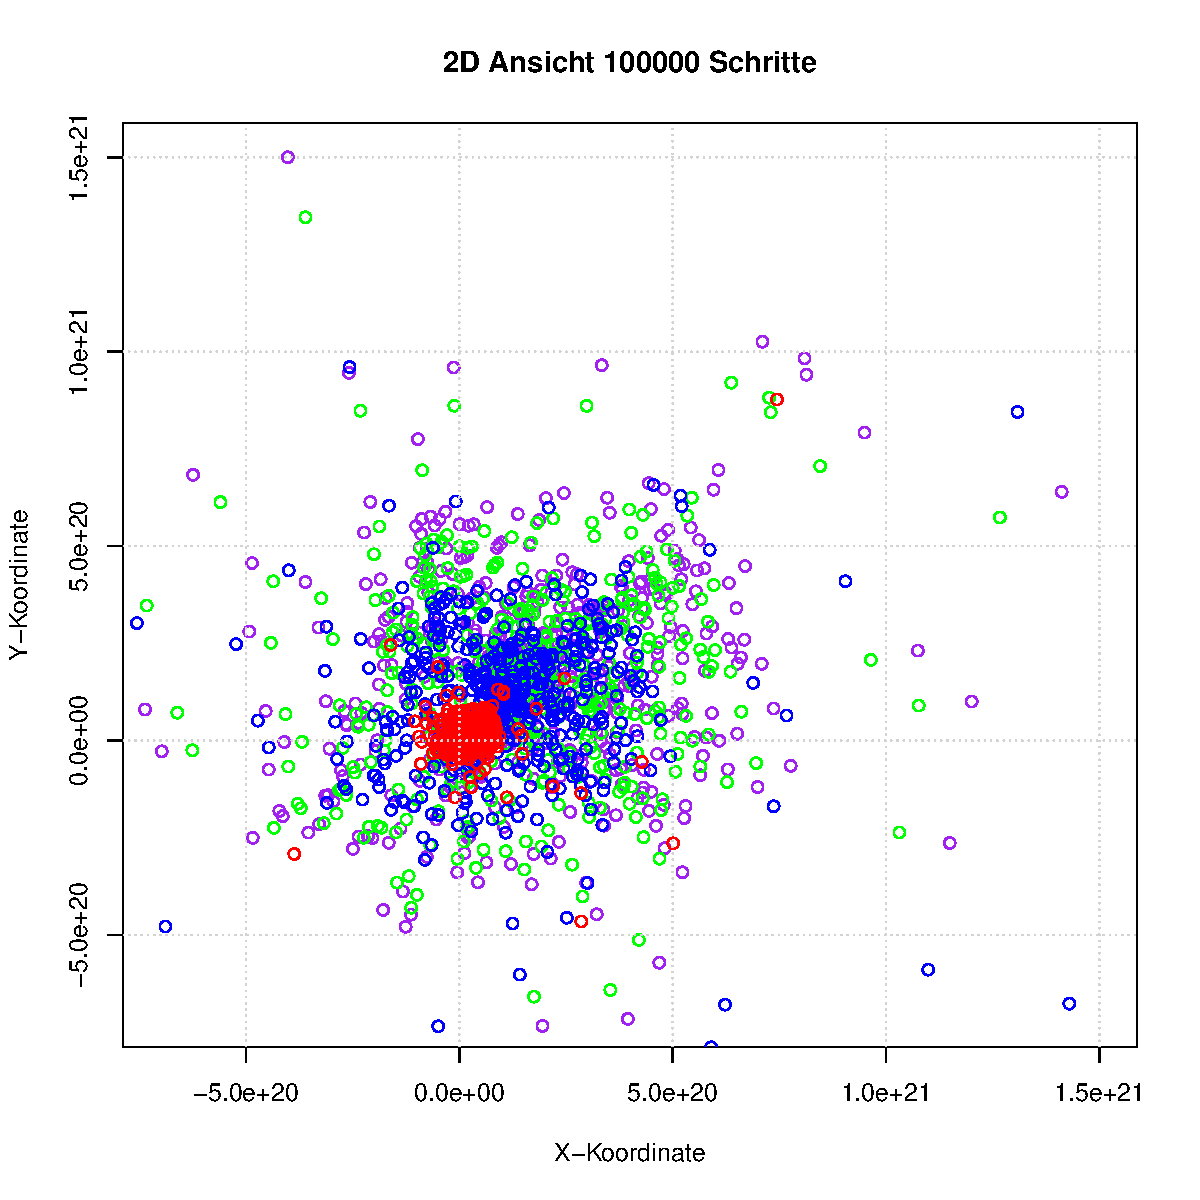
\includegraphics[width = 8cm]{kugel/images/verschiebung.pdf}
	\end{center}
	\caption{Impulsproblem
	\label{Kugel.Impulsproblem}}
\end{figure}

Zur Korrektur dieser Unsch"onheit haben wir diese beiden Formeln implementiert:
\begin{equation}
	 P = \sum m_i  v_i \qquad  v_{i+1} =  v_i - \dfrac{ P}{n \cdot m_i}
	\label{kugel:Formel:Korrektur}
\end{equation}
Zuerst wird der Gesamtimpuls des Haufens berechnet. Aus diesem folgt
ein durchschnittlicher Impuls pro Stern, mit dem dann schlussendlich
die Geschwindigkeit eines Sterns korrigiert wird. Dadurch wird der
Gesamtimpuls des Kugelsternhaufens auf 0 gesetzt und somit bleibt er an
Ort und Stelle stehen. Folgend noch der Code daf"ur:
\begin{Cpp}
for (int i = 0 ; i < anzahlSterne ; i++){	// Gesamtimpuls berechnen
	m = s[i].getMass();
	impuls[0] += s[i].getSpeedX() * m;
	impuls[1] += s[i].getSpeedY() * m;
	impuls[2] += s[i].getSpeedZ() * m;
}
  
impuls[0] /= anzahlSterne;					// Impuls pro Stern
impuls[1] /= anzahlSterne;
impuls[2] /= anzahlSterne;

for (int i = 0 ; i < anzahlSterne ; i++){	// Korrektur 
	m = s[i].getMass();
	buff = s[i].getSpeedX() - impuls[0]/m;
	s[i].setSpeedX(buff);
	buff = s[i].getSpeedY() - impuls[1]/m;
	s[i].setSpeedY(buff);
	buff = s[i].getSpeedZ() - impuls[2]/m;
	s[i].setSpeedZ(buff);
}
\end{Cpp}	
	
\subsection{Umgang mit Daten}
Positionen, mittlere Energie sowie auch der mittlere Radius (Abstand
zum Mittelpunkt des Haufens) der Sterne werden in \texttt{csv-Files}
gespeichert. Zur Auswertung wurden mittels dem Programm \texttt{R}
Plots erstellt. Es war dabei schwierig die richtige Gr"osse der
\texttt{csv-Files} festzulegen, weil sie werden bei langer Laufzeit
unhandlich gross. Wir mussten uns daher eine Strategie zur Verteilung
der Daten in verschieden Files zurechtlegen, wof"ur folgende Fragen
adressiert worden sind:
\begin{enumerate}
\item Die Resultate wie vieler Zeitschritte sollen in einem File
gespeichert werden?
\item Werden Kennzahlen (Energie, Radius) in separaten Files
gespeichert?
\index{Energie}

Nach mehreren Versuchen entschlossen wir uns ins File
\texttt{Data\#\#\#.csv} die Koordinaten des f"unften Sternes
(zum Verfolgen eines einzelnen Sterns), den durchschnittlichen
Radius und die Energie des Kugelsternhaufens nach jeweils 100
Zeitschritten zu speichern. Nach 10'000 Schritten (100 Eintr"age)
wird dieses File abgeschlossen und die Files \texttt{Pos\#\#\#.csv} und
\texttt{Rad\#\#\#.csv} werden generiert, dabei werden im \texttt{Pos-File}
die Positionen aller Sterne und im \texttt{Rad-File} alle Radien (sofern
sie kleiner als $\mathrm{10^{30}}$ sind) gespeichert. Diese Begrenzung
des Radius soll verhindern dass Sterne die aus dem Haufen geschleudert
werden die Auswertung verf"alschen k"onnen.
\item Wie sollen die vielen Files benannt werden?

Wir generieren dazu einen dynamischen String der durch eine Z"ahlvariable
File f"ur File ver"andert wird. Im folgenden Codebeispiel sieht man wie
der Name eines Pos-Files, sowie das File selber erstellt werden. Dazu muss
beachtet werden dass die Z"ahlvariable \texttt{fileCount} ausserhalb der
Methode \texttt{saveAllStars(Stern* s)} jeweils nach 10'000 Zeitschritten
inkrementiert wird.
\end{enumerate}
\begin{Cpp}
void saveAllStars(Stern* s) {
  char buffer[1024];
  snprintf(buffer, sizeof(buffer), "Pos%09d.csv", fileCount);
  ofstream data;
  data.open(buffer);			          // Filestream oeffnen
  data << "x,y,z" << endl;
  for(int x=0 ; x<anzahlSterne ; x++){    // Koordinaten ins File schreiben
    data << s[x].getCordX() << "," << s[x].getCordY() << "," << s[x].getCordZ() << endl;
  }
  data.close();				         	  // Filestream schliessen
}
\end{Cpp}
Solange man nur zwei Wochen lang simuliert kann man die Daten so
abspeichern, jedoch nach l"angerer Zeit werden es etwas viele Dateien. Im
Nachhinein w"are es besser gewesen f"ur die lange Simulation nur jeden
500sten Schritt in das \texttt{Data-File} zu speichern und alle 1'000'000
Schritte die Positionen und Radien abspeichern.

\section{Fazit}
\rhead{Fazit}
Alles in allem gelang es uns nicht einen stabilen Kugelsternhaufen
zu simulieren. Die Sterne fliegen zum Teil ineinander hindurch ohne
aufeinander einzuwirken. Das hat mit einem viel zu gross gew"ahltem
Zeitschritt zu tun. Wird dieser allerdings verringert, so hat das
massive Auswirkungen auf die Simulationszeit. Je mehr Sterne man hat,
desto kleiner sollte auch der Zeitschritt sein.
In unseren letzten Simulationsversuchen haben wir nur noch mit 1000
Sternen gerechnet, allerdings war der Zeitschritt mit f"unf Jahren immer
noch viel zu gross.
In einem letzten Versuch, der bei Abschluss dieser Arbeit bereits sieben
Wochen am Laufen war, probieren wir den Haufen durch einen station"aren
grossen Massenpunkt, also ein Schwarzes Loch sozusagen, zu stabilisieren.
Man kann schon ein "ahnliches Verhalten wie bei einem realen
Kugelsternhaufen erkennen, allerdings wird er nicht wirklich rund wie
man in der Abbildung~\ref{Kugel.FormKug} erkennen kann.
\begin{figure}[h!]
\begin{center}
		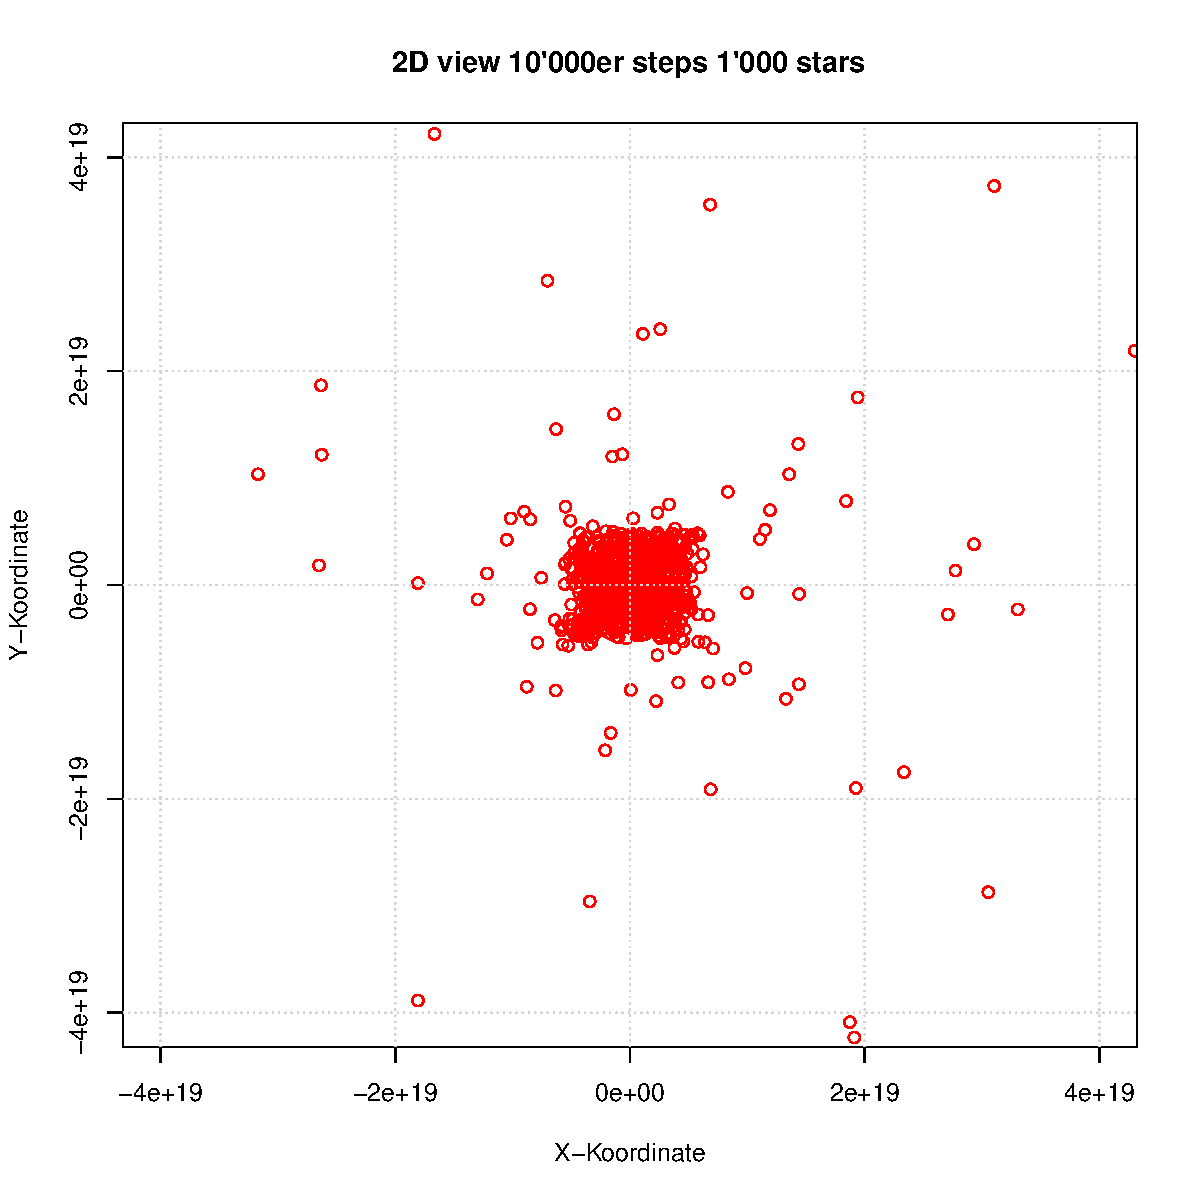
\includegraphics[width = 8cm]{kugel/images/quadrat.pdf}
\end{center}
\caption{Form Kugelsternhaufen
\label{Kugel.FormKug}}
\end{figure}\\

\printbibliography[heading=subbibliography]
\end{refsection}
